\chapter{Logic view}
I dette kapitel beskrives systemets forskellige logiske komponenter.

\section{Overblik}
Weplanners software kan overordnet set opdeles i 3 pakker. Et billede af dette kan ses på figur \ref{fig:Weplanner_overview}.  


\begin{figure}[H]
    \centering
    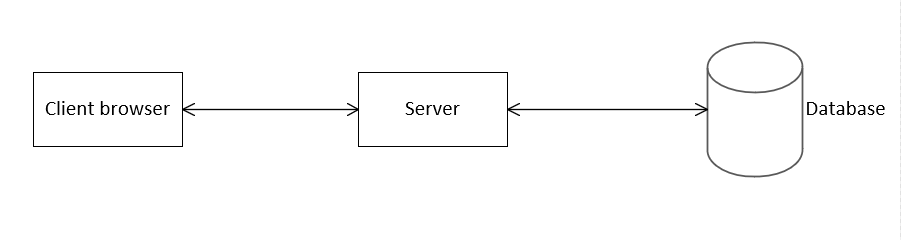
\includegraphics[scale=0.5]{05_Arkitektur/Images/LogicView.png}
    \caption{Overblik over weplanners software}
    \label{fig:Weplanner_overview}
\end{figure}

Serveren er i vores tilfælde den egentlige computer der bestemmer hvordan det hele kommer til at se ud. Ud fra en forespørgsel fra en klient, sender den HTML og JS ud til klienten via en HTTPS forbindelse. Brugeren kan ved hjælp af interfacet kommunikere med serveren. Alt efter hvilken forespørgsel som serveren modtager, opdaterer den databasen eller henter data fra den og sender det ud til brugeren.

